% !TeX spellcheck = <engl>

\let\textcircled=\pgftextcircled

\chapter{Results and Analysis}
\label{chap:results}

Following the described methodology in the previous chapter, this chapter seeks to interpret and analyse the results obtained while evaluating 


\section{Can We Automatically Detect Scene Contexts?}
\subsection{Metrics}
In evaluating the classifiers, it was  crucial to understand the predictive power of the two context classifiers. As such, precision, recall and f1-score were selected as the main performance metrics. 
\paragraph{Precision} is the percentage of positive predictions that were correct. 
\begin{equation*}
\centering
Precision=\frac{TP}{TP+FP}
\end{equation*}
\paragraph{Recall} is the percentage of positive samples that were correctly predicted. 
\begin{equation*}
\centering
Recall=\frac{TP}{TP+FN}
\end{equation*}
\paragraph{F1-score} is the balanced mean of the precision and recall.  
\begin{equation*}
\centering 
2\cdot\frac{precision\cdot recall}{precision+recall}
\end{equation*}
\subsection{Analysis}

I established that determining the context from images is much more accurate than from point clouds. As highlighted before, images offer higher representational power and resolution than sparse point clouds. As seen in figure 41, the f1-score of the image classifier outperformed the point cloud classifier by more than 30\% . 


\begin{table}[h] % Context detection
	\centering
	\resizebox{\textwidth}{!}{%
		\begin{tabular}{|
				>{\columncolor[HTML]{FFFFFF}}l |
				>{\columncolor[HTML]{FFFFC7}}l |
				>{\columncolor[HTML]{FFFFC7}}l |
				>{\columncolor[HTML]{FFFFC7}}l |
				>{\columncolor[HTML]{FFFFC7}}l |
				>{\columncolor[HTML]{96FFFB}}l |
				>{\columncolor[HTML]{96FFFB}}l |
				>{\columncolor[HTML]{96FFFB}}l |
				>{\columncolor[HTML]{96FFFB}}l |}
			\hline
			{\color[HTML]{333333} \textbf{}} & \multicolumn{4}{l|}{\cellcolor[HTML]{FFFFC7}{\color[HTML]{333333} \textbf{Context Detection using PointCloud Feature Matching}}} & \multicolumn{4}{l|}{\cellcolor[HTML]{96FFFB}\textbf{Context Detection using Image Segmentation}} \\ \hline
			{\color[HTML]{333333} \textbf{Context}} & {\color[HTML]{333333} \textbf{precision}} & {\color[HTML]{333333} \textbf{recall}} & {\color[HTML]{333333} \textbf{f1-score}} & {\color[HTML]{333333} \textbf{support}} & \textbf{precision} & \textbf{recall} & \textbf{f1-score} & \textbf{support} \\ \hline
			{\color[HTML]{333333} \textit{\textbf{urban}}} & {\color[HTML]{333333} \textbf{0.52}} & {\color[HTML]{333333} 0.45} & {\color[HTML]{333333} 0.48} & {\color[HTML]{333333} 206} & 0.81 & \textbf{0.9} & \textbf{0.85} & 193 \\ \hline
			{\color[HTML]{333333} \textit{\textbf{non-urban}}} & {\color[HTML]{333333} 0.51} & {\color[HTML]{333333} \textbf{0.58}} & {\color[HTML]{333333} \textbf{0.55}} & {\color[HTML]{333333} 206} & \textbf{0.9} & 0.81 & \textbf{0.85} & 218 \\ \hline
			{\color[HTML]{333333} \textbf{avg / total}} & {\color[HTML]{333333} 0.51} & {\color[HTML]{333333} 0.51} & {\color[HTML]{333333} 0.51} & {\color[HTML]{333333} 412} & 0.86 & 0.85 & 0.85 & 411 \\ \hline
		\end{tabular}%
	}
	\caption{Comparison of context detection methods}
	\label{my-label}
\end{table}

With regard to the point cloud context classifier, majority voting resulted in around 50:50 precision for both classes. The recall for the non-urban was 7 percent more than urban which was below 50\%. By implementing the penalty function in the point cloud classifier, recall for the urban class improved by 17\%  as seen in table \ref{tab:penalisedpcl}. 

\begin{table}[h] % Penalised
	\centering
	\begin{tabular}{|l|l|l|l|l|}
		\hline
		\multicolumn{5}{|l|}{\textbf{Penalised Point Cloud Context Classifier}}                            \\ \hline
		\textbf{context}            & \textbf{precision} & \textbf{recall} & \textbf{f1-score} & \textbf{support} \\ \hline
		\textbf{urban}       & \textbf{0.52}      & \textbf{0.62}   & \textbf{0.54}     & 206              \\ \hline
		\textbf{non-urban}   & 0.46               & 0.33            & 0.38              & 206              \\ \hline
		\textbf{avg / total} & 0.47               & 0.47            & 0.46              & 412              \\ \hline
	\end{tabular}
	\caption{Penalised Point Cloud classifier}
	\label{tab:penalisedpcl}
\end{table}

\section{Do Object Detection Models Perform Better in Different Contexts?}
\subsection*{Metrics}
\subsubsection*{KITTI Evaluation Protocol}
The models were evaluated using the official KITTI evaluation protocol. Average precision(AP) is the area under a recall-precision curve that was calculated after predictions. Predicted bounding boxes were considered as positive matched if they were above a predefined intersection over union(IoU). 
IoU is calculated as: \\ 
\begin{math}
\centering
IoU = \frac{Overlap\, area}{Union\, area}
\end{math} \\ 
Where the overlap area is the region that is shared between the predicted bounding box and the ground truth bounding box and the Union area is the total area of the predicted bounding box and ground truth box.
This was calculated for 2D bounding boxes, 3D bounding boxes and Bird-Eye View bounding boxes. The IoU threshold was set at  $\geq$0.7 for the car class and $\geq$0.5 for the pedestrian class. 

\subsubsection*{GPU}
As mentioned earlier, the resources of an AV are limited and therefore it is encouraged to implement efficient models. In light of this, I monitored the GPU statistics to better understand how different models affect the GPU. 
During inference, GPU statistics were collected at an interval of 1 second using NVIDIA System Management Interface(nvidia-smi). The following metrics were collected. 
\begin{itemize}[noitemsep]
	\item \textbf{Power Draw } - Watts
	\item \textbf{Memory Used } - MB
	\item \textbf{Temperature} - $\degree$C
	\item \textbf{Clock Speed} - MHz
\end{itemize}
For uniformity purposes, all the experiments were performed on single NVIDIA P100 GPU with 16GB High Bandwidth Memory. 
\subsubsection*{Baseline}
 A baseline, was established by running each model was run on the original KITTI validation dataset. The results can be seen in table  in \ref{tab:baseline}. In addition, the temperature and power metrics were collected and can be seen in the last boxplot of figures \ref{fig:temp} and \ref{fig:power}.

\begin{table}[h] %baseline
	\centering
	\resizebox{\textwidth}{!}{%
		\begin{tabular}{|l|l|
				>{\columncolor[HTML]{FFCCC9}}l |
				>{\columncolor[HTML]{FFCCC9}}l |
				>{\columncolor[HTML]{FFCCC9}}l |
				>{\columncolor[HTML]{96FFFB}}l |
				>{\columncolor[HTML]{96FFFB}}l |
				>{\columncolor[HTML]{96FFFB}}l |}
			\hline
			& \textbf{Class}                     & \multicolumn{3}{l|}{\cellcolor[HTML]{FFCCC9}{\color[HTML]{000000} \textbf{Car}}}                                                  & \multicolumn{3}{l|}{\cellcolor[HTML]{96FFFB}{\color[HTML]{000000} \textbf{Pedestrian}}}                                           \\ \hline
			\textbf{Model}               & \textbf{Difficulty}                & {\color[HTML]{000000} \textbf{Easy}}      & {\color[HTML]{000000} \textbf{Medium}}    & {\color[HTML]{000000} \textbf{Hard}}      & {\color[HTML]{000000} \textbf{Easy}}      & {\color[HTML]{000000} \textbf{Medium}}    & {\color[HTML]{000000} \textbf{Hard}}      \\ \hline
			& \textit{\textbf{2D Bounding Box}}  & {\color[HTML]{000000} \textbf{86.987999}} & {\color[HTML]{000000} \textbf{77.10569}}  & {\color[HTML]{000000} \textbf{68.012459}} & {\color[HTML]{000000} 56.214417}          & {\color[HTML]{000000} 51.969517}          & {\color[HTML]{000000} 46.578247}          \\ \cline{2-8} 
			& \textit{\textbf{BEV Bounding Box}} & {\color[HTML]{000000} \textbf{86.00412}}  & {\color[HTML]{000000} \textbf{74.355942}} & {\color[HTML]{000000} \textbf{65.62397}}  & {\color[HTML]{000000} \textbf{50.94368}}  & {\color[HTML]{000000} \textbf{49.857227}} & {\color[HTML]{000000} \textbf{44.704525}} \\ \cline{2-8} 
			\multirow{-3}{*}{\textbf{AVOD}}     & \textit{\textbf{3D Bounding Box}}  & {\color[HTML]{000000} \textbf{75.447769}} & {\color[HTML]{000000} \textbf{63.742085}} & {\color[HTML]{000000} \textbf{54.334251}} & {\color[HTML]{000000} \textbf{48.757492}} & {\color[HTML]{000000} \textbf{44.84359}}  & {\color[HTML]{000000} \textbf{43.014023}} \\ \hline
			& \textit{\textbf{2D Bounding Box}}  & {\color[HTML]{000000} 65.951279}          & {\color[HTML]{000000} 56.683437}          & {\color[HTML]{000000} 55.972511}          & {\color[HTML]{000000} \textbf{66.309807}} & {\color[HTML]{000000} \textbf{60.556213}} & {\color[HTML]{000000} \textbf{53.479141}} \\ \cline{2-8} 
			& \textit{\textbf{BEV Bounding Box}} & {\color[HTML]{000000} 81.242409}          & {\color[HTML]{000000} 70.672707}          & {\color[HTML]{000000} 65.347595}          & {\color[HTML]{000000} 50.308723}          & {\color[HTML]{000000} 46.726196}          & {\color[HTML]{000000} 41.24551}           \\ \cline{2-8} 
			\multirow{-3}{*}{\textbf{VoxelNet}} & \textit{\textbf{3D Bounding Box}}  & {\color[HTML]{000000} 40.000149}          & {\color[HTML]{000000} 34.892159}          & {\color[HTML]{000000} 31.376112}          & {\color[HTML]{000000} 34.161884}          & {\color[HTML]{000000} 30.576441}          & {\color[HTML]{000000} 28.982103}          \\ \hline
		\end{tabular}%
	}
	\caption{Baseline}
	\label{tab:baseline}
\end{table}

\subsubsection{Running Each Model Exclusively}
To investigate whether the performance of each model varies in different contexts, each model was run exclusively on a single GPU with data from each context dataset. 

\begin{table}[h] %Car AP
	\centering
	\resizebox{\textwidth}{!}{%
		\begin{tabular}{|l|l|
				>{\columncolor[HTML]{FFCCC9}}l |
				>{\columncolor[HTML]{FFCCC9}}l |
				>{\columncolor[HTML]{FFCCC9}}l |
				>{\columncolor[HTML]{96FFFB}}l |
				>{\columncolor[HTML]{96FFFB}}l |
				>{\columncolor[HTML]{96FFFB}}l |}
			\hline
			\textbf{}                           & \textbf{Context}                   & \multicolumn{3}{l|}{\cellcolor[HTML]{FFCCC9}\textbf{Urban}}  & \multicolumn{3}{l|}{\cellcolor[HTML]{96FFFB}\textbf{Non-Urban}} \\ \hline
			\textbf{Model}                           & \textbf{Difficulty}                & \textbf{Easy}      & \textbf{Medium}    & \textbf{Hard}      & \textbf{Easy}       & \textbf{Medium}     & \textbf{Hard}       \\ \hline
			\multirow{3}{*}{\textbf{AVOD}} & \textit{\textbf{2D Bounding Box}} & \textbf{86.987999} & \textbf{77.10569} & \textbf{68.012459} & \textbf{89.186172} & \textbf{79.754562} & \textbf{78.550514} \\ \cline{2-8} 
			& \textit{\textbf{BEV Bounding Box}} & 86.00412 & 74.355942 & 65.62397 & 87.11274 & \textbf{76.859818} & \textbf{75.720955} \\ \cline{2-8} 
			& \textit{\textbf{3D Bounding Box}} & \textbf{75.447769} & \textbf{63.742085} & \textbf{54.334251} & \textbf{75.430656} & \textbf{64.199951} & \textbf{62.902302} \\ \hline
			\multicolumn{1}{|c|}{\multirow{3}{*}{\textbf{VoxelNet}}} & \textit{\textbf{2D Bounding Box}} & 69.597939 & 65.98201 & 59.284454 & 77.520409 & 67.733231 & 62.281651 \\ \cline{2-8} 
			\multicolumn{1}{|c|}{} & \textit{\textbf{BEV Bounding Box}} & \textbf{86.34037} & \textbf{76.187859} & \textbf{68.103294} & \textbf{88.635025} & 75.361214 & 69.502548 \\ \cline{2-8} 
			\multicolumn{1}{|c|}{} & \textit{\textbf{3D Bounding Box}} & 73.632263 & 58.473991 & 50.744587 & 68.620865 & 49.455608 & 45.809917 \\ \hline
		\end{tabular}%
	}
	\caption{Car AP}
	\label{tab:cardetap}
\end{table}
\begin{table}[h]%Pedestrian AP
	\centering
	\resizebox{\textwidth}{!}{%
		\begin{tabular}{|l|l|
				>{\columncolor[HTML]{FFCCC9}}l |
				>{\columncolor[HTML]{FFCCC9}}l |
				>{\columncolor[HTML]{FFCCC9}}l |
				>{\columncolor[HTML]{96FFFB}}l |
				>{\columncolor[HTML]{96FFFB}}l |
				>{\columncolor[HTML]{96FFFB}}l |}
			\hline
			\textbf{}                           & \textbf{Context}                   & \multicolumn{3}{l|}{\cellcolor[HTML]{FFCCC9}\textbf{Urban}}  & \multicolumn{3}{l|}{\cellcolor[HTML]{96FFFB}\textbf{Non-Urban}} \\ \hline
			\textbf{Model}                           & \textbf{Difficulty}                & \textbf{Easy}      & \textbf{Medium}    & \textbf{Hard}      & \textbf{Easy}       & \textbf{Medium}     & \textbf{Hard}       \\ \hline
			& \textit{\textbf{2D Bounding Box}}  & \textbf{78.626633} & \textbf{77.407684} & \textbf{70.029228} & 76.096977           & 70.946465           & 71.205276           \\ \cline{2-8} 
			& \textit{\textbf{BEV Bounding Box}} & \textbf{80.880447} & \textbf{80.393105} & \textbf{79.296593} & 77.806831           & 77.654358           & 71.792923           \\ \cline{2-8} 
			\multirow{-3}{*}{\textbf{AVOD}}     & \textit{\textbf{3D Bounding Box}}  & \textbf{80.649719} & \textbf{80.142876} & \textbf{79.056778} & 77.538368           & 71.868484           & 71.564285           \\ \hline
			& \textit{\textbf{2D Bounding Box}}  & 72.129387          & 65.245384          & 65.508232          & \textbf{84.218407}  & \textbf{76.52832}   & \textbf{76.593803}  \\ \cline{2-8} 
			& \textit{\textbf{BEV Bounding Box}} & 74.766678          & 73.944069          & 74.138588          & \textbf{89.830276}  & \textbf{80.201164}  & \textbf{80.114815}  \\ \cline{2-8} 
			\multirow{-3}{*}{\textbf{VoxelNet}} & \textit{\textbf{3D Bounding Box}}  & 71.177628          & 64.247559          & 64.18145           & \textbf{87.206612}  & \textbf{77.964493}  & \textbf{78.036652}  \\ \hline
		\end{tabular}%
	}
	\caption{Pedestrian AP}
	\label{tab:pedap}
\end{table}
\begin{table}[h]%Time
	\centering
	%	\resizebox{\textwidth}{!}{%
	\begin{tabular}{|l|l|l|l|l|l|l|}
		\hline
		\multirow{2}{*}{\textbf{Context}} & \multicolumn{3}{l|}{\textbf{VoxelNet}} & \multicolumn{3}{c|}{\textbf{AVOD}} \\ \cline{2-7} 
		& \textbf{min} & \textbf{max} & \textbf{mean} & \textbf{min} & \textbf{max} & \textbf{mean} \\ \hline
		\textbf{Urban} & 0.113 & 3.813 & 0.129 & \textbf{0.095} & \textbf{2.457} & \textbf{0.112} \\ \hline
		\textbf{Non-urban} & 0.113 & \textbf{2.224} & 0.127 & \textbf{0.096} & 2.506 & \textbf{0.113} \\ \hline
	\end{tabular}%
	%	}
	\caption{Inference Time on Single NVIDIA P100 GPU}
	\label{tab:inftime}
\end{table}
\begin{figure}[h] %Power&Temp
	\centering
	\begin{minipage}[b]{0.7\textwidth}
		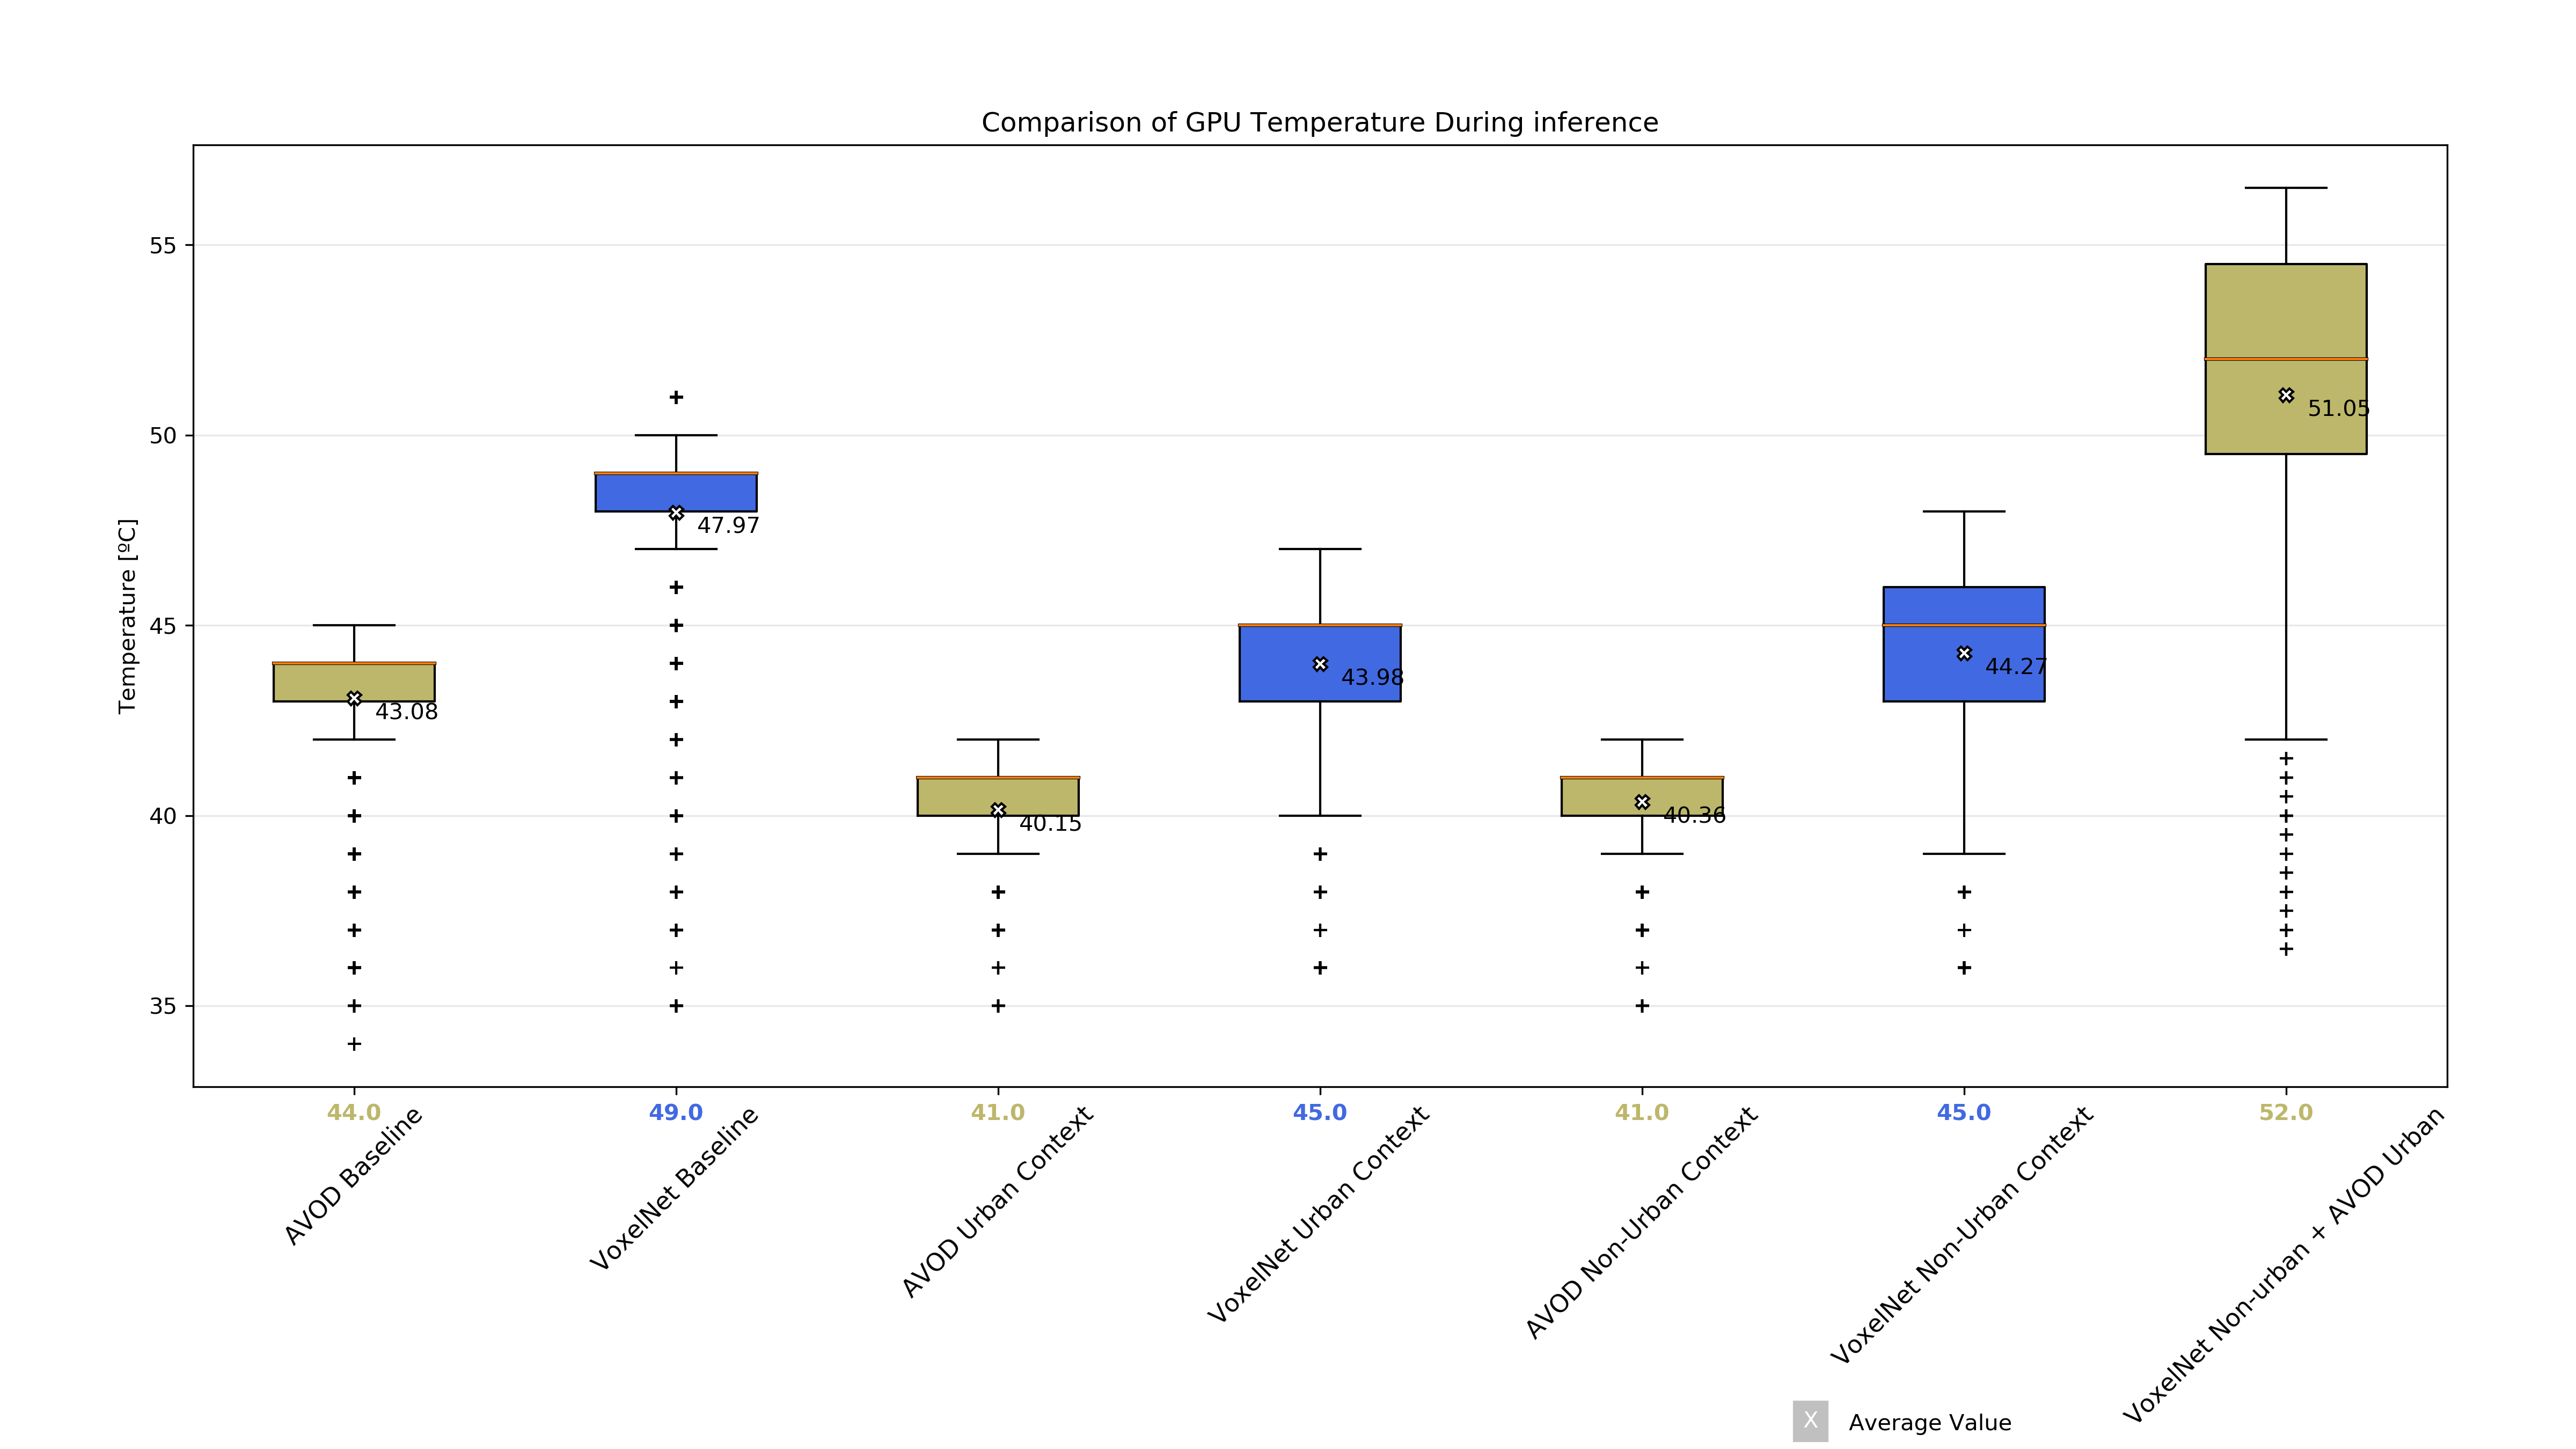
\includegraphics[width=\textwidth]{images/gputepbox.png}
		\caption{Temperature boxplots of evaluation runs.Voxelnet(blue) AVOD(gold) AVOD+VoxelNet(Red)}
		\label{fig:temp}
	\end{minipage}
	%	\hfill
	\begin{minipage}[b]{0.7\textwidth}
		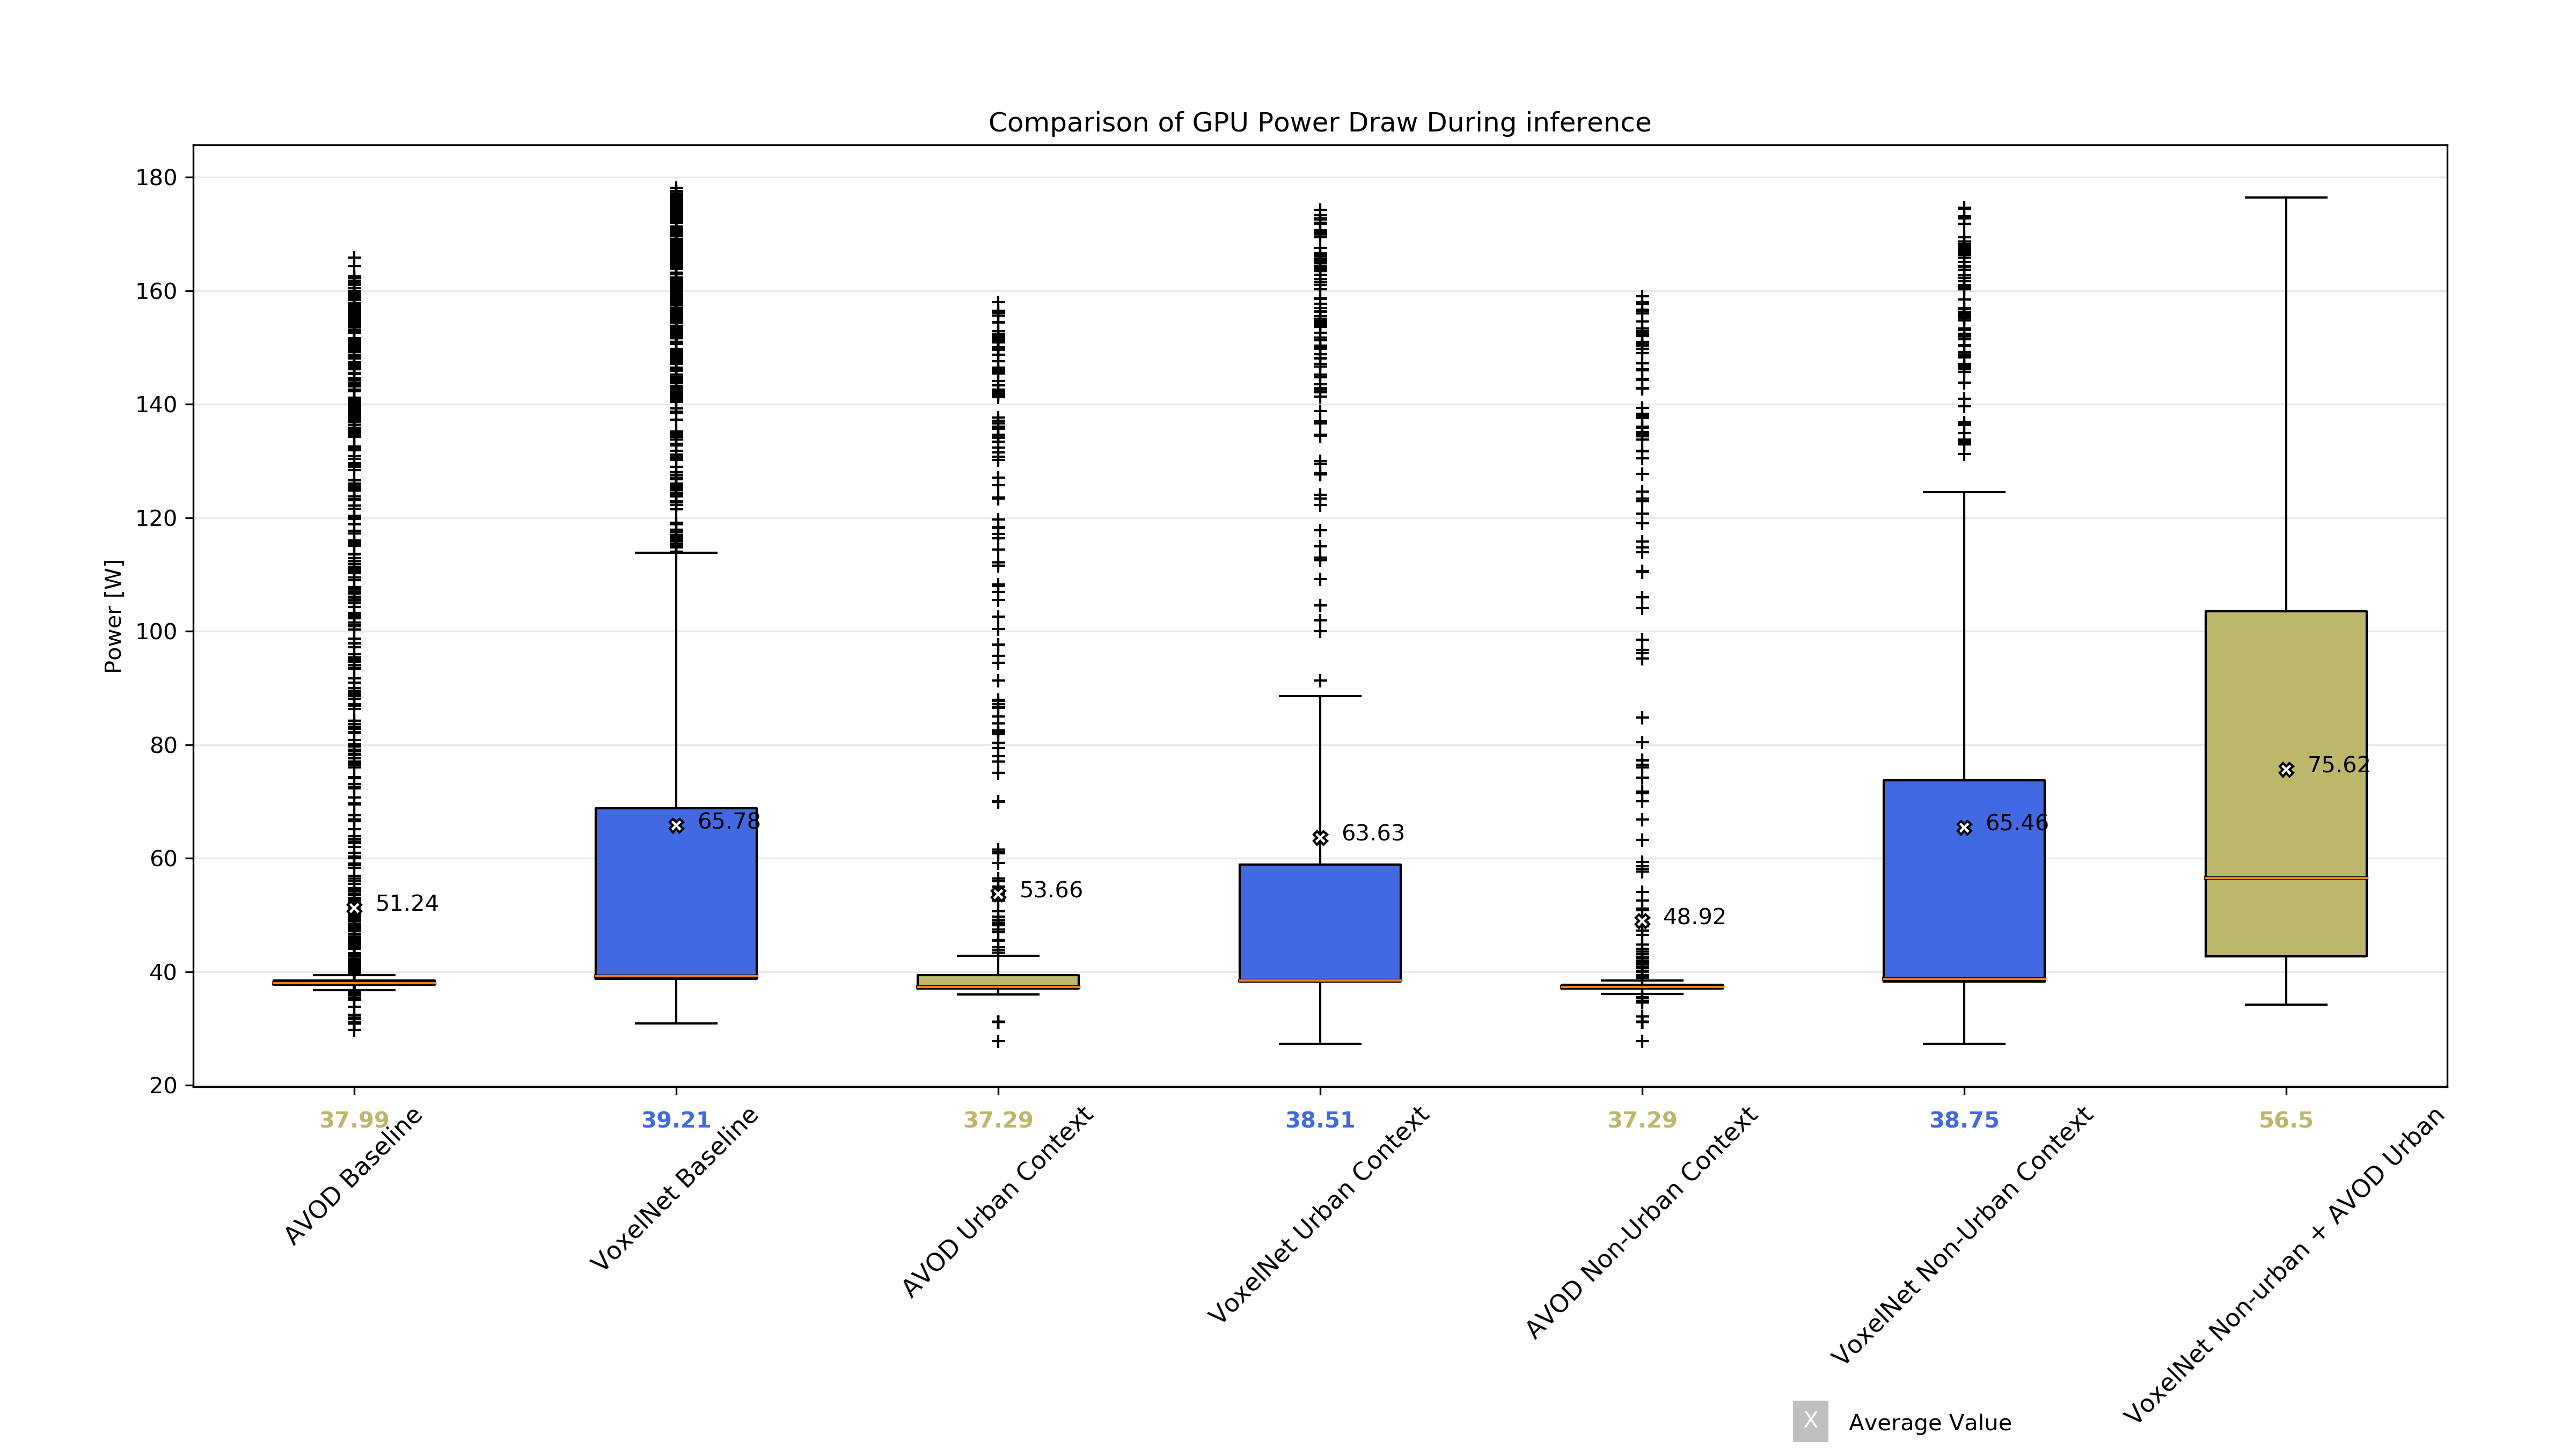
\includegraphics[width=\textwidth]{images/gpupbox.png}
		\caption{Power boxplots of evaluation runs. Voxelnet(blue), AVOD(gold), AVOD+VoxelNet(Red}
		\label{fig:power}
	\end{minipage}
	
\end{figure}


\subsubsection*{Analysis}
\paragraph{Car} - AVOD outperformed VoxelNet on 2D and 3D detections in both contexts. However, VoxelNet performed slightly better in bird-eye-view detections as compared to AVOD. 
\paragraph{Pedestrian} - As compared to the car class, there was a distinct performance boundary whereby AVOD dominated all detections in the urban context whereas VoxelNet did in the non-urban context.

It is important to bear in mind that for the car class, the IoU threshold for detections is 0.7 as compared to the pedestrian IoU threshold of 0.5. As mentioned earlier while describing the model architectures, due to the fact that AVOD fuses the top proposals from the image and LiDAR point cloud feature maps, the predicted bounding boxes tend to be tighter and thus have a higher IoU. Going by the pedestrian class result, it is plausible to argue that the performance of VoxelNet would have been higher or close to AVOD's given that the IoU threshold was slightly reduced. 

\paragraph{GPU} - As seen in figures \ref{fig:power} and \ref{fig:temp},AVOD generally ran at a lower temperature and consumed less power as compared to VoxelNet.In fact, temperature-wise, VoxelNet ran hotter over 75\% of the time.  Furthermore, AVOD's temperature and power usage varied less  as compared to VoxelNet's which fluctuated along a larger range. 
With regard to context, by only running the models on a specific context dataset, power usage and temperature decreased for both VoxelNet and AVOD. 

\subsubsection*{Running Both Models Simultaneously}
Having identified that AVOD is better at detecting cars and pedestrians in urban contexts and VoxelNet in non-urban contexts, I set out to further investigate whether it is possible to have both models running on a single GPU. 

\begin{table}[H] % memory
	\centering
	\caption{Memory}
	\label{tab:mem}
	\begin{tabular}{|l|l|l|}
		\hline
		& \textbf{Min} & \textbf{Max} \\ \hline
		\textbf{Memory(MB)} & 4608.50  & 14320.00\\ \hline
	\end{tabular}
	
\end{table}


\subsubsection*{Analysis}

\paragraph{Temperature} - Running both models simultaneously resulted in significantly higher temperatures as compared running them exclusively. The average temperature was 7\degree hotter than the maximum mean temperature from running the models exclusively. 
\paragraph{Power} - Similarly, the mean power usage was 10 watts greater than  the maximum mean power from running the models exclusively. 
\paragraph{Memory} - Running both models resulted in a total memory usage of 14.3 GB out of the total memory of 16GB thereby proving that they are able to run optimally on a GPU with 16GB+ memory.  


\section{Is VoxelNet Performance Valid For Different Datasets?}
\subsection*{Metrics}
Given that the data was collected from a stationary vehicle in an urban area with mostly pedestrians,  VoxelNet was evaluated on the pedestrian class only. However, as there was no corresponding image data for the point clouds, only the 3D bounding boxes and Bird-Eye View bounding boxes with IoU $\geq$ 0.5. were used in calculating the AP. 
\subsection*{Analysis}
VoxelNet was not able to predict any objects on the SIL dataset. As highlighted before, the VLP-16 LiDAR sensor has a lower frequency than that of the HDL-64E. This therefore affected the point cloud density and is visible in figure \ref{fig:difference} . SIL point clouds had an average point cloud density per frame that was lower than that of KITTI's by 42\%  in 1000 samples as seen in figure \ref{fig:density}. This was evaluated by calculating the number of points in each point cloud frame and dividing by the frame size. It is therefore safe to conclude that the point cloud density has a positive correlation to the performance of LiDAR only models. 


\begin{figure}[H] %SIL KITTI
	\centering
	\begin{minipage}[b]{0.49\textwidth}
		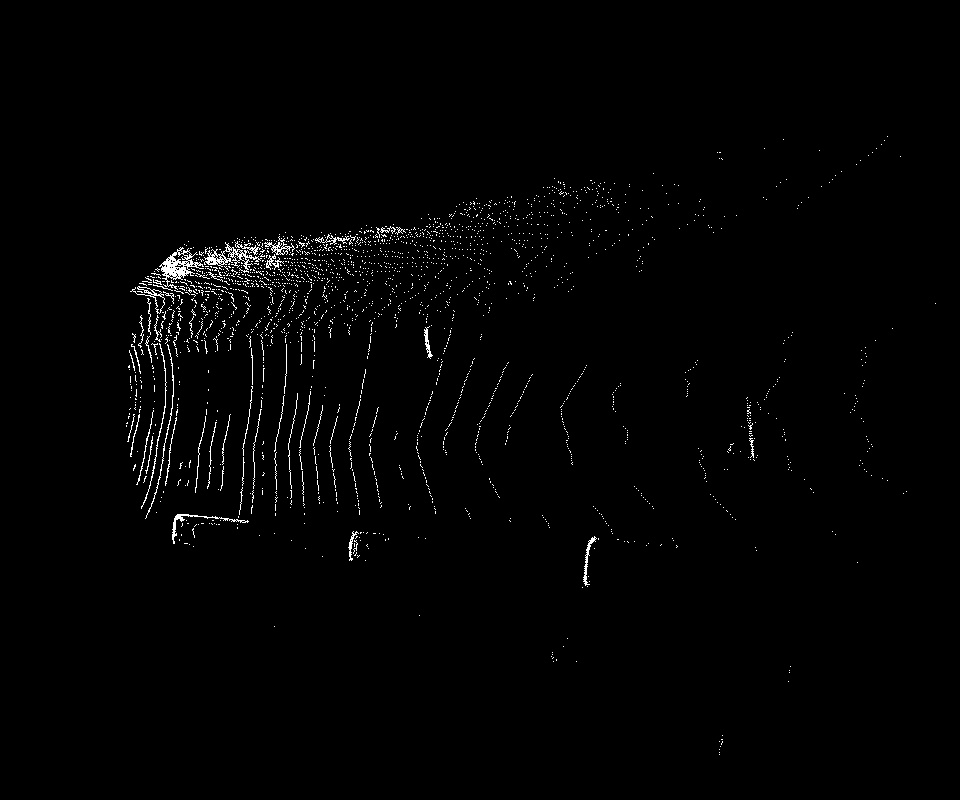
\includegraphics[width=\textwidth,height=6.5cm]{images/kitti_bv}
		\caption*{KITTI bird eye view}
%		\label{fig:kittibv}
	\end{minipage}
	%	\hfill
	\begin{minipage}[b]{0.49\textwidth}
		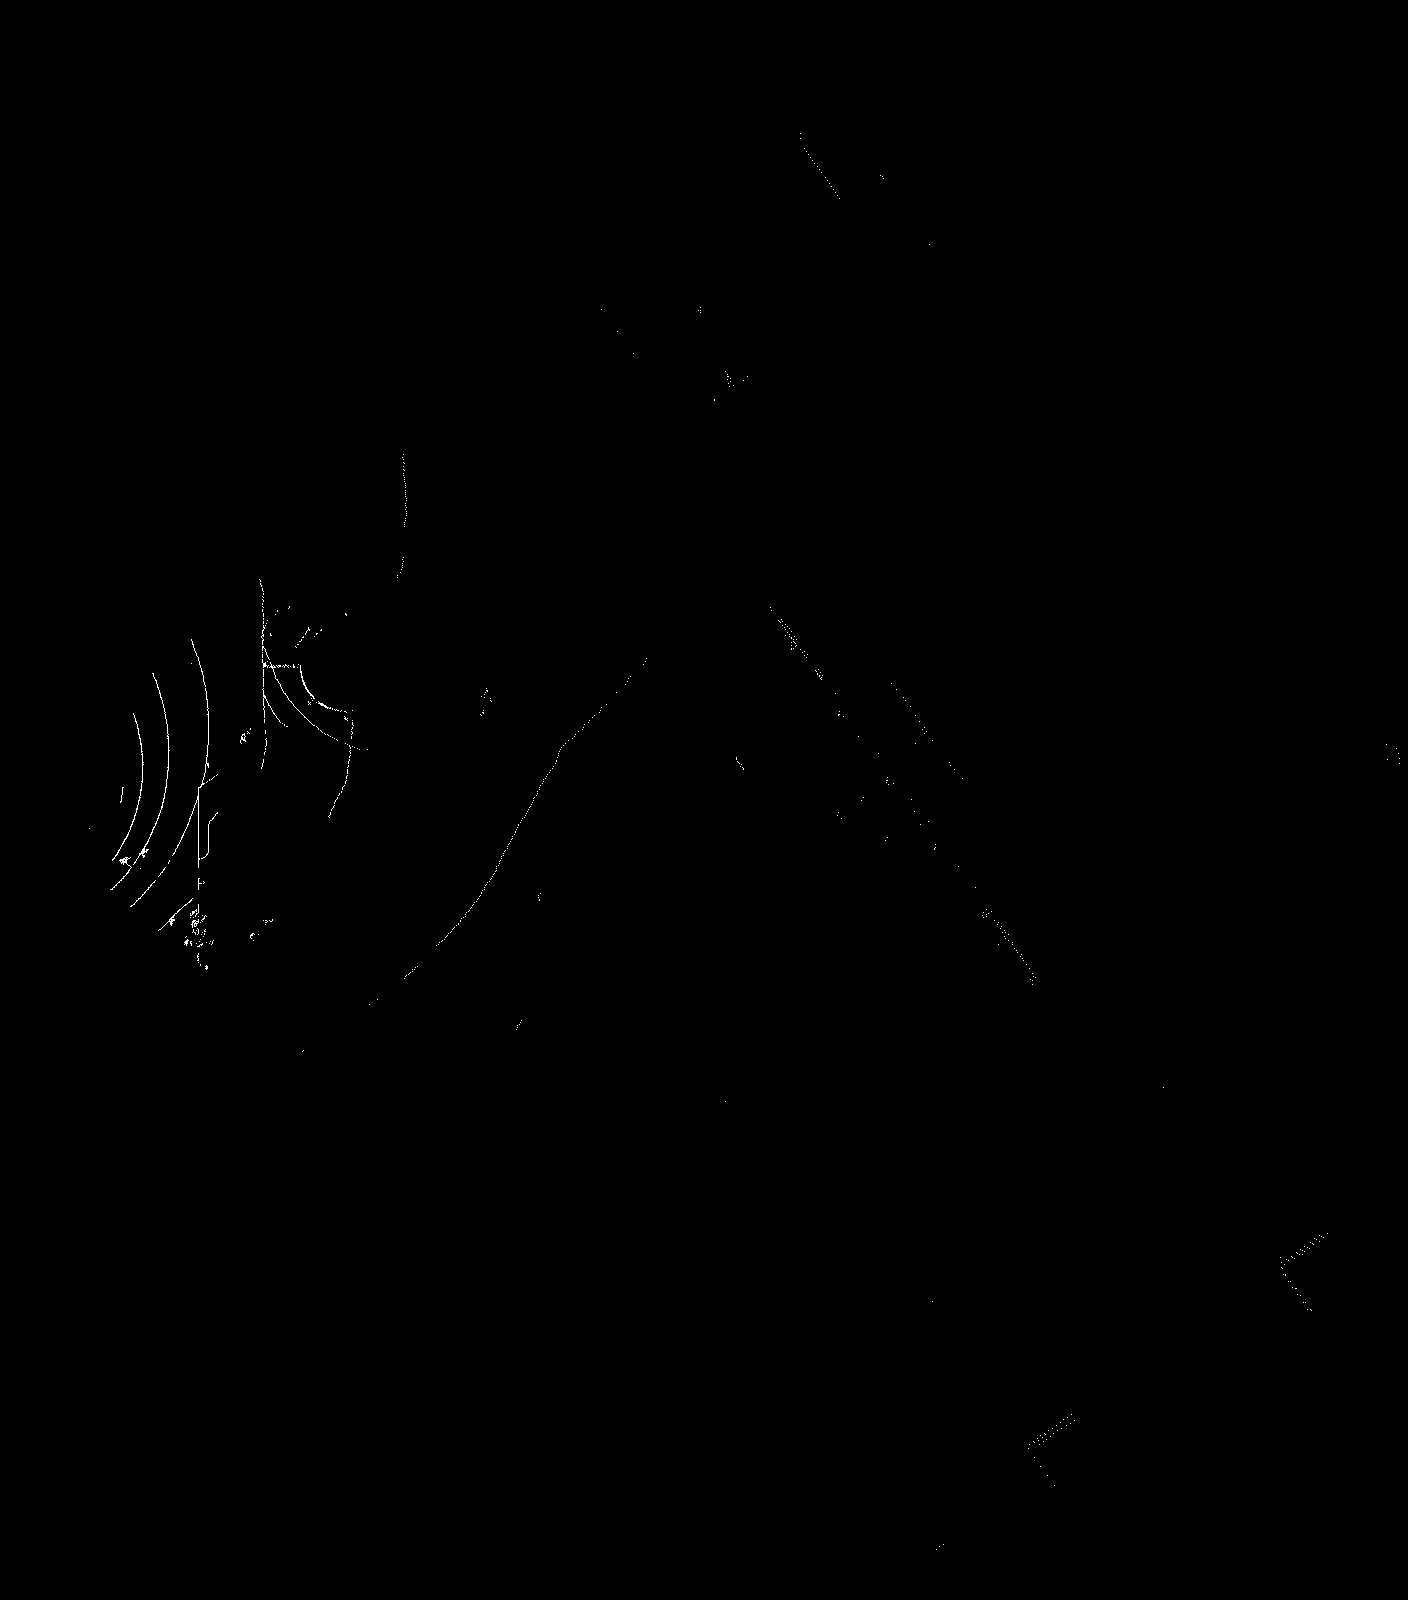
\includegraphics[width=\textwidth,height=6.5cm]{images/sil_bv}
		\caption*{SIL bird eye view}
%		\label{fig:silbv}
	\end{minipage}
	\caption{Bird Eye View Difference between SIL and KITTI}
	\label{fig:difference}
\end{figure}

\begin{figure}[H] % density
	\centering
	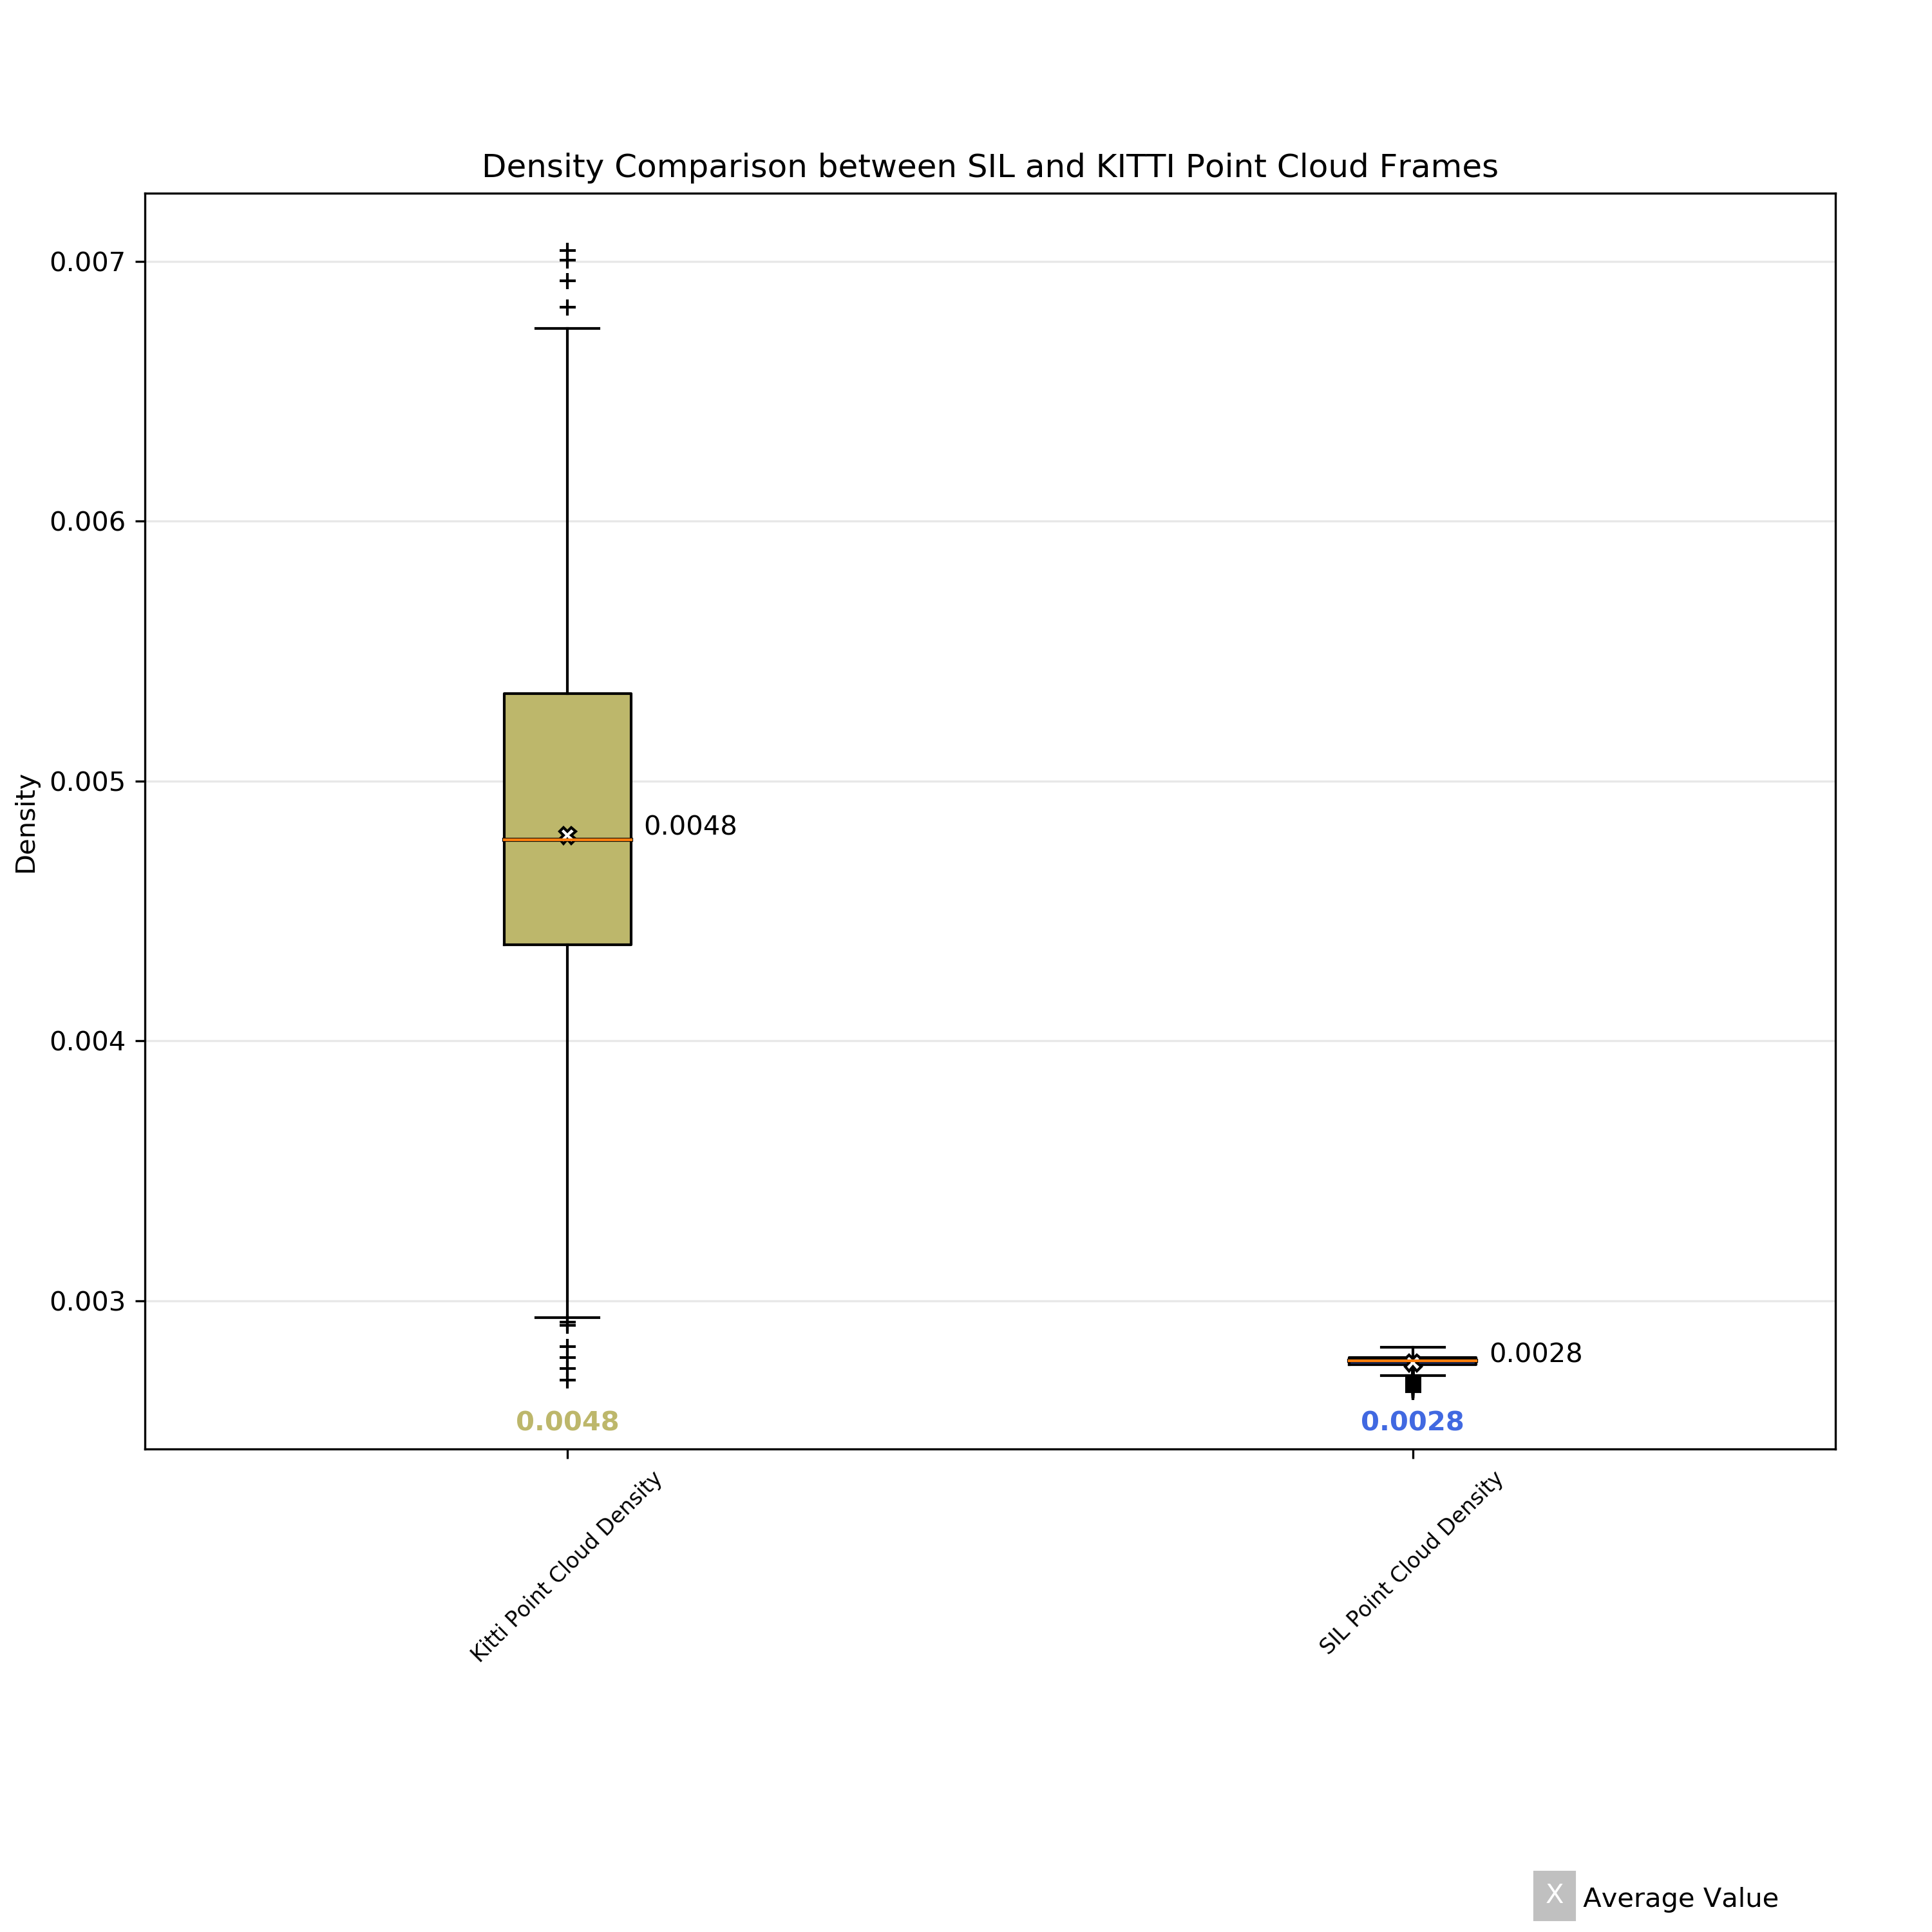
\includegraphics[width=0.6\linewidth]{images/density}
	\caption{Point Cloud Density}
	\label{fig:density}
\end{figure}